\documentclass{article}
\usepackage{listings}
\usepackage{mathrsfs}
\usepackage[utf8]{inputenc}
\usepackage{amssymb}
\usepackage{lipsum}
\usepackage{amsmath}
\usepackage{fancyhdr}
\usepackage{geometry}
\usepackage{scrextend}
\usepackage[english,german]{babel}
\usepackage{titling}
\setlength{\droptitle}{-3cm}
\usepackage{tikz}
\usepackage{algorithm,algpseudocode}
\usepackage[doublespacing]{setspace}
\usetikzlibrary{datavisualization}
\usetikzlibrary{datavisualization.formats.functions}
\usepackage{polynom}
\usepackage{amsmath}
\usepackage{gauss}
\usepackage{tkz-euclide}
\usetikzlibrary{datavisualization}
\usetikzlibrary{datavisualization.formats.functions}
\author{
Alexander Mattick Kennung: qi69dube\\
Kapitel 1
}
\usepackage{import}
\date{\today}
\geometry{a4paper, margin=2cm}
\usepackage{stackengine}
\parskip 1em
\newcommand\stackequal[2]{%
  \mathrel{\stackunder[2pt]{\stackon[4pt]{=}{$\scriptscriptstyle#1$}}{%
  $\scriptscriptstyle#2$}}
 }
\makeatletter
\renewcommand*\env@matrix[1][*\c@MaxMatrixCols c]{%
  \hskip -\arraycolsep
  \let\@ifnextchar\new@ifnextchar
  \array{#1}}
\makeatother
\lstset{
  language=haskell,
}
\lstnewenvironment{code}{\lstset{language=Haskell,basicstyle=\small}}{}
\usepackage{enumitem}
\setlist{nosep}
\usepackage{titlesec}

\titlespacing*{\subsection}{0pt}{2pt}{3pt}
\titlespacing*{\section}{0pt}{0pt}{5pt}
\titlespacing*{\subsubsection}{0pt}{1pt}{2pt}
\title{Vorlesung 4}


\begin{document}
	\maketitle
	traceroute ist immer roundtrip\\
	\section{2.3}
	Leitungsvermittlung bei konstanten daten in regelmäßigen abschnitten\\
	Flußkontrolle vermeidet überlastung des Ziels.\\
	Überlast verhindert überlastung des Netzes zwischen Sender/Ziel\\
	\\
	Gegeben:\\
	$R=1Mbps$, $R_{gen} = 64kbps, d_{prop}=2ms, L=48Bytes$\\
	$d_{gen}=\frac{48*8bit}{64000bps}=0.006=6ms$ ,\\
	$d_{trans}=\frac{48*8bit}{1000 000bps}=384\mu s$\\
	$d_{ges}= 2ms+6ms+384\mu s\approx 2ms$\\
	\section{2.4}
	Pro $\frac{NL}{R}$ kommen N pakete hinzu, ausgehende übertragungsrate $R$, Paketgröße $L$\\
	Das erste Paket hat keine Warteschlangeverzögerung.\\
	Das zweite $1\frac{L}{R}$.\\
	Das dritte $2\frac{L}{R}$\\
	$d_i$ ist $d_{queue}$ des i-ten pakets.\\
	$d_{ges}$ warteschlangeverzögerung pro periode\\
	$d_i = (i-1)\frac{L}{R}$
	$\sum\limits^{n-1}_{i=1} i\frac{L}{R} = \frac{(N-1)NL}{2R}$\\
	$\overline{d} = \frac{(n-1)L}{2R}$\\
	für N=4: $\frac{3L}{2R}$\\
	\section{2.5}
	$d_{prop}+d_{queue} = \frac{L}{R}+\frac{L\rho}{R(1-\rho)} =\frac{L}{R}(1+\frac{\rho}{(1-\rho)}) $\\
	$\frac{L}{R}(1+\frac{\rho}{(1-\rho)})=\frac{L}{R(1-\rho)}=\frac{L}{R}\frac{1}{1-\frac{\lambda L}{R}}=\frac{L}{R(1-\lambda\frac{L}{R})}$\\
	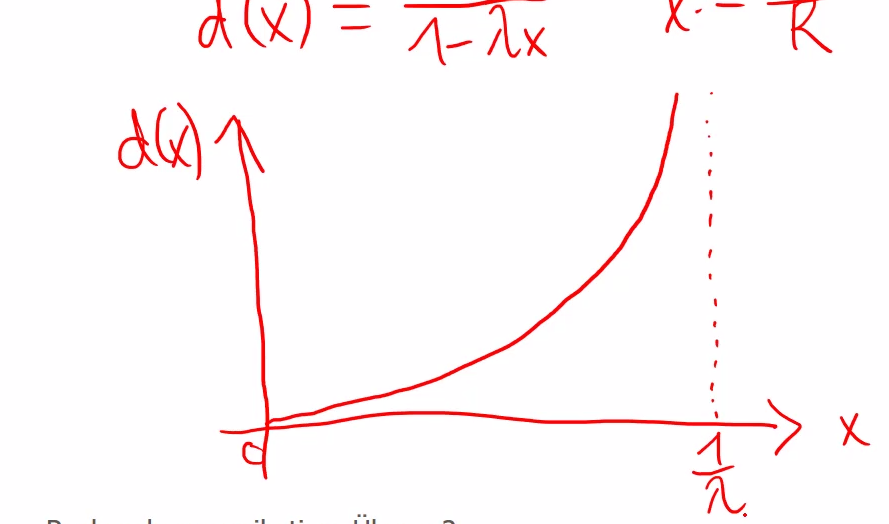
\includegraphics[scale=0.25]{warteschlangenplot.png}\\
	$\lambda$ ist ankunftsrate in pakete pro sekunde.\\
	für homogene Netze gilt:\\
	$d_{end-end} = E(d_{proc}+d_{trans}+d_{prop})+d_{proc,dst}$\\
	für heterogene %nimmt man einfach die durchschnittliche verzögerung pro link:
	%$d_{end-end} = E(\mathbb{E}_{d\simp(x)}[\d_{proc}+d_{trans}+d_{prop}])+d_{proc,dst}$\\
	\\
	$d_{end-end} = \sum\limits_{i=1}^E(\d_{proc,i}+d_{trans,i}+d_{prop,i})+d_{proc,dst}$\\
\end{document}